\chapter{The Power of the Dot} % (fold)
\label{chap:The Power of the Dot}
In object-oriented languages, the receiver of an operation usually precedes the
dot. As described in section~\ref{sec:Placing the Receiver at the End}, this
has some downsides. However, it also brings advantages: The IDE can help you
find the correct method because the syntax "|receiver.|" allows the IDE to list
all operations of the receiver's type! \cite[Ch. "The Power of the
Dot"]{frege_goodness} \\ 
This chapter shows how one can exploit the module
system of JavaScript to get similar suggestions from the IDE, even when not
working with objects!

\section{The JavaScript Module System} % (fold)
\label{sec:The JavaScript Module System}

Nowadays, when JavaScript programs are increasingly complex, it makes sense to
structure the code better. Modules are a great way to do this - they define
clear interfaces in which things are made available to other modules.
For a JavaScript file to become a module, it must either
\begin{itemize}
  \item export part of its functionalities using |export|
  \item or import functionality from other modules via |import|.
\end{itemize}

Listing~\ref{lst:js_module_example} shows an example of a simple JavaScript
module:
\begin{lstlisting}[
  style=ES6,
  caption=A simple JavaScript module,
  label={lst:js_module_example}
]
import { Sequence } from "../src/sequence/sequence.js"; *'\label{line:js_module_example1}'*

export { endlessSeq }

const incrFn     = i => i + 1;
const whileFn    = _ => true;
const endlessSeq = Sequence(0, whileFn, incrFn);
\end{lstlisting}

Listing~\ref{lst:js_module_example} imports the constructor |Sequence| and
becomes a module. It exports |endlessSeq|, which then becomes available in
other modules. |incrFn| and |whileFn| are not exported and, therefore, only
available in this module.
% subsection The JavaScript Module System (end)

\subsection{IDE Support through modules} % (fold)
\label{sub:IDE support through modules}
The module system offers several possibilities to bring autocompletion to
the IDE using the dot.
\subsubsection{Named Imports} % (fold)
\label{subsub:Named Imports}
The Sequence library offers many loose functions. To use them, you need to know
their names. This is not easy, especially for beginners, and reduces the
development speed. Fortunately, this can be solved using named imports.
Line~\ref{line:named_imports_js1} in listing~\ref{lst:named_imports_js} imports
the Sequence library with the name "|_|":

\begin{lstlisting}[
  style=ES6,
  caption=Named imports in JavaScript,
  label={lst:named_imports_js}
]
import *'\colorbox{code-highlight}{* as \_}'* from "../src/sequence/sequence.js" *'\label{line:named_imports_js1}'*

const seq = *'\colorbox{code-highlight}{\_.}'*Sequence(0, i => i < 5, i => i + 1);*'\label{line:named_imports_js2}'*

console.log(_.show(seq));
// => Logs '[0,1,2,3,4]'
\end{lstlisting}
This allows the developer to access exported symbols of "|_|" using "|_.|".
Thanks to the "|.|" (dot) after the module name (|_|), IDEs like IntelliJ IDEA
will suggest exported members of this module.\\
Figure~\ref{fig:the_power_of_the_dot_idea_sugg} shows exactly this behaviour:

\begin{figure}[H]
  \begin{center}
    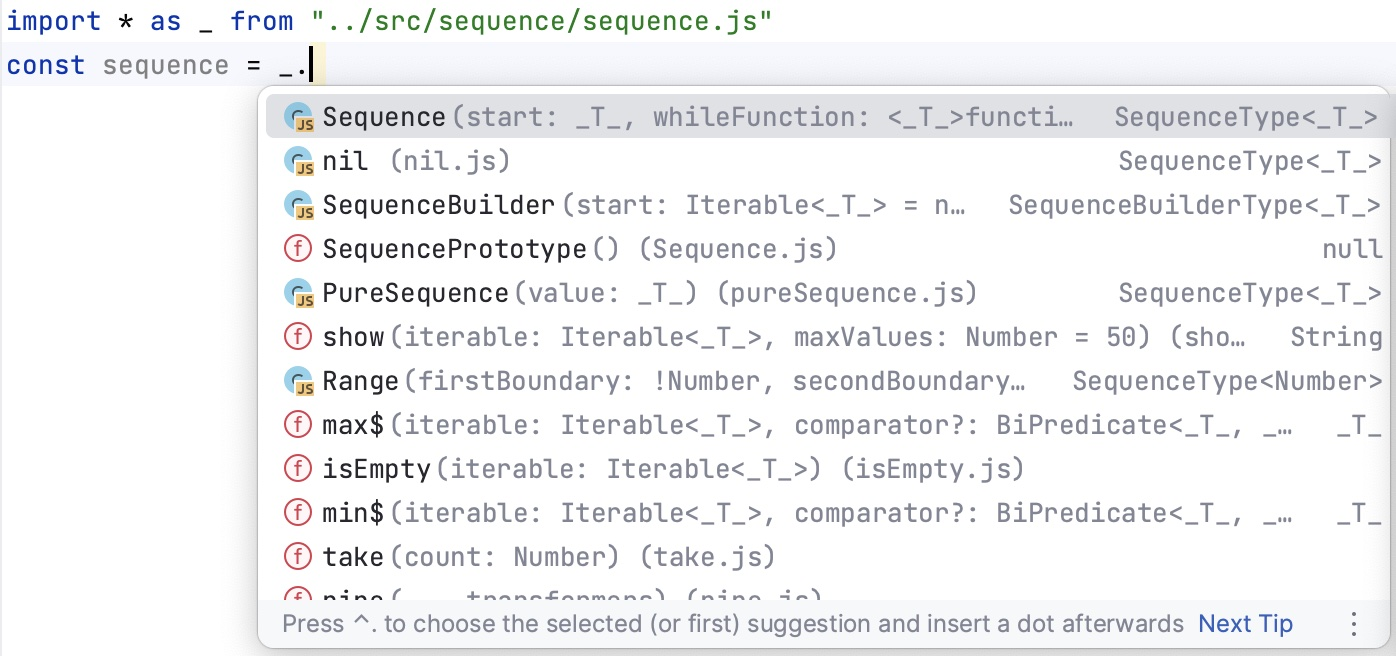
\includegraphics[width=0.95\textwidth]{mainmatter/pictures/the-power-of-the-dot-intellj.jpg}
  \end{center}
  \caption{IntelliJ suggests exported members of a named import}
  \label{fig:the_power_of_the_dot_idea_sugg}
\end{figure}

This is a way to combine the power of the dot with the advantages of placing
the receiver at the end! \\
For users who know the library well, typing the additional name represents an
unnecessary extra effort. The good thing about named imports is that every
export supports them - the library developer does not need to adapt the
exports. \\
This leaves it up to the user to import the library named! Named
imports, therefore, allow the flexible customization of module names.

Additionally, object destructuring allows using often used symbols without
module names as listing~\ref{lst:destr_named_import} shows:

\begin{lstlisting}[
  style=ES6,
  caption=Destructuring of a named import,
  label={lst:destr_named_import}
]
import *'\colorbox{code-highlight}{* as \_}'* from "../src/sequence/sequence.js" 
const { Sequence, show } = *'\colorbox{code-highlight}{\_}'*; *'\label{line:destr_named_import1}'*

const seq = Sequence(0, i => i < 5, i => i + 1); *'\label{line:destr_named_import3}'*

console.log(show(seq));
// => Logs '[0,1,2,3,4]'
\end{lstlisting}

The statement on line~\ref{line:destr_named_import1} destructures the named
module. Thus, |Sequence| is available as if a developer had imported it
typically.


% subsubsection Named Imports (end)
\subsection{The Namespace Object Pattern} % (fold)
\label{sub:The Namespace Object Pattern}
The previously described approach with named imports is great for
functionalities that are only loosely related. What do you do if you want to
define modules that share a common interface with other modules? Good examples
of such a use case are services. Often you use dummy services in unit tests
that should have the same interface as the production services that access an
API. The Namespace Object pattern solves this problem!

Listing~\ref{lst:namespace_object} defines a service with two methods. The
object |service| gathers these two methods into a single namespace. This object
is the only thing that the module exports.

\begin{lstlisting}[
  style=ES6,
  caption=The Namespace Object pattern,
  label={lst:namespace_object}
]
export { service }

const getAll  = () => { /* <omitted> */ };
const getById = id => { /* <omitted> */ };

const service = { getAll, getById };
\end{lstlisting}

A user of this service can now import it very easily, as
listing~\ref{lst:import_namespace_obj} shows:

\begin{lstlisting}[
  style=ES6,
  caption=Import a Namespace Object,
  label={lst:import_namespace_obj}
]
import { service } from "./power-of-the-dot.js";

const allElements = service.getAll();
\end{lstlisting}

Since this object can follow a defined interface (for example, using JSDoc), it
can easily be replaced by just changing the import to another implementation.
% subsubsection The Namespace object pattern (end)

\subsubsection{Conclusion} % (fold)
\label{subsub:Power_of_the_dot_Conclusion}
The module system of JavaScript offers several possibilities to couple
loose functions. While namespace objects can fulfil an interface, the
flexibility of named imports makes it easier for developers to get started with
a potentially comprehensive library. \\ 
Both approaches allow the IDE to provide the developer with additional support by
bringing "the power of the dot" to JavaScript modules!

% subsubsection Conclusion (end)
% subsection IDE support through modules (end)
% section The Power of the Dot (end)
